%; whizzy section -pdf xpdf -latex ./whizzypdfptex.sh
% latex beamer presentation.
% platex, latex-beamer でコンパイルすることを想定。

%     Tokyo Debian Meeting resources
%     Copyright (C) 2007 Junichi Uekawa

%     This program is free software; you can redistribute it and/or modify
%     it under the terms of the GNU General Public License as published by
%     the Free Software Foundation; either version 2 of the License, or
%     (at your option) any later version.

%     This program is distributed in the hope that it will be useful,
%     but WITHOUT ANY WARRANTY; without even the implied warranty of
%     MERCHANTABILITY or FITNESS FOR A PARTICULAR PURPOSE.  See the
%     GNU General Public License for more details.

%     You should have received a copy of the GNU General Public License
%     along with this program; if not, write to the Free Software
%     Foundation, Inc., 51 Franklin St, Fifth Floor, Boston, MA  02110-1301 USA

\documentclass[cjk,dvipdfmx,12pt]{beamer}
\usetheme{Tokyo}
\usepackage{ulem}
\usepackage{tabularx}

\usepackage{fancybox}
\usepackage{fancyvrb}
\usepackage{float}
\usepackage[english]{babel}
% commandline環境を定義。画面入出力についてはcommandline環境
% で表記する
\newenvironment{commandline}%
{\VerbatimEnvironment
  \begin{Sbox}\begin{minipage}{0.9\hsize}\begin{fontsize}{7.3}{7.3} \begin{BVerbatim}}%
{\end{BVerbatim}\end{fontsize}\end{minipage}\end{Sbox}
  \setlength{\fboxsep}{8pt}
% start on a new paragraph

\vspace{6pt}% skip before
\fcolorbox{dancerdarkblue}{dancerlightblue}{\TheSbox}

\vspace{6pt}% skip after
}
%end of commandline

\definecolor{dancerdarkblue}{rgb}{0,0.08,0.45}
\definecolor{dancernormalblue}{rgb}{0.8,0.9,0.95}
\definecolor{dancerlightblue}{rgb}{0.8,0.95,1}


%  preview (shell-command (concat "evince " (replace-regexp-in-string "tex$" "pdf"(buffer-file-name)) "&"))
%  presentation (shell-command (concat "xpdf -fullscreen " (replace-regexp-in-string "tex$" "pdf"(buffer-file-name)) "&"))

%http://www.naney.org/diki/dk/hyperref.html
%日本語EUC系環境の時
\AtBeginDvi{\special{pdf:tounicode EUC-UCS2}}
%シフトJIS系環境の時
%\AtBeginDvi{\special{pdf:tounicode 90ms-RKSJ-UCS2}}

\title{東京エリア Debian 勉強会}
\subtitle{資料}
\author{上川 純一 dancer@debian.org\\IRC nick: dancerj}
\date{2007年12月15日}
\logo{
\includegraphics[width=8cm]{image200607/openlogo-light.eps}}


% 間のタイトルページ用
\newcommand{\emtext}[1]{
\begin{frame}{}

\begin{minipage}{0.55\hsize}
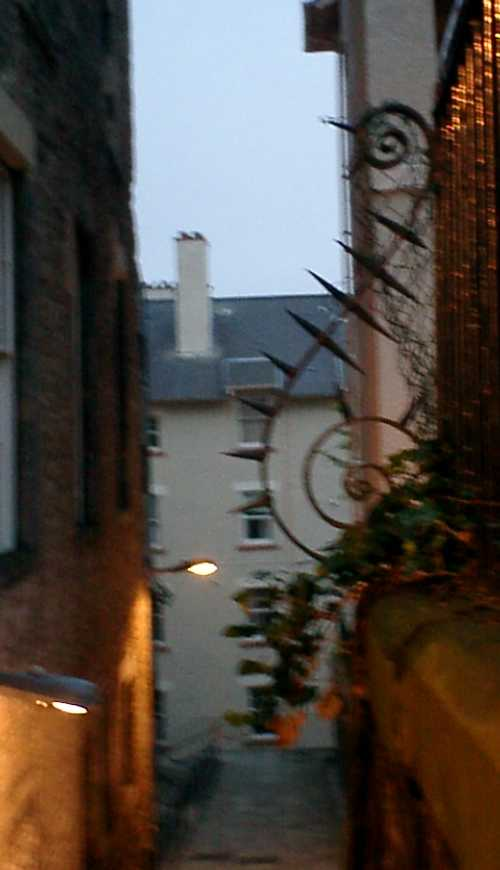
\includegraphics[width=1\hsize]{image200707/gurutitle.jpg}
\end{minipage}
\begin{minipage}{0.39\hsize}
 {\Huge #1
 }
\end{minipage}
\end{frame}
}

% 三択問題用
\newcounter{santakucounter}
\newcommand{\santaku}[5]{%
\addtocounter{santakucounter}{1}
\frame{\frametitle{問題\arabic{santakucounter}. #1}
%問題\arabic{santakucounter}. #1
\begin{minipage}[t]{0.8\hsize}
 \begin{itemize}
 \item
      \begin{minipage}{0.2\hsize}
      
\includegraphics[width=0.9\hsize]{image200703/janken-A.png}\end{minipage}
       \begin{minipage}{0.6\hsize}
       A #2\end{minipage}\\
 \item
      \begin{minipage}{0.2\hsize}
      
\includegraphics[width=0.9\hsize]{image200703/janken-B.png}\end{minipage}
       \begin{minipage}{0.6\hsize}
       B #3\end{minipage}\\
 \item
      \begin{minipage}{0.2\hsize}
      
\includegraphics[width=0.9\hsize]{image200703/janken-C.png}\end{minipage}
       \begin{minipage}{0.6\hsize}
       C #4\end{minipage}\\
 \end{itemize}
\end{minipage}
}
\frame{\frametitle{問題\arabic{santakucounter}. #1}
%問題\arabic{santakucounter}. #1
\begin{minipage}[t]{0.8\hsize}
\begin{itemize}
 \item
      \begin{minipage}{0.2\hsize}
      
\includegraphics[width=0.9\hsize]{image200703/janken-A.png}\end{minipage}
       \begin{minipage}{0.6\hsize}
       A #2\end{minipage}\\
 \item
      \begin{minipage}{0.2\hsize}
      
\includegraphics[width=0.9\hsize]{image200703/janken-B.png}\end{minipage}
       \begin{minipage}{0.6\hsize}
       B #3\end{minipage}\\
 \item
      \begin{minipage}{0.2\hsize}
      
\includegraphics[width=0.9\hsize]{image200703/janken-C.png}\end{minipage}
       \begin{minipage}{0.6\hsize}
       C #4\end{minipage}\\
\end{itemize}
\end{minipage}
\begin{minipage}[t]{0.15\hsize}
答えは:

\vspace{1cm}

  {\huge \hspace{1cm}#5}
  \hspace{-6cm}\includegraphics[width=4cm]{image200703/janken-#5.png}
 \end{minipage}}
}

\begin{document}
\frame{\titlepage{}}

\section{Intro}

\emtext{設営準備にご協力ください}

\begin{frame}
 \frametitle{Agenda}
\begin{minipage}[t]{0.45\hsize}
  \begin{itemize}
  \item 注意事項
	\begin{itemize}
	 \item 飲食禁止
	 \item 政治/宗教/営利活動禁止
	\end{itemize}
  \item quiz
  \item 最近のDebian関連のイベント
	\begin{itemize}
	 \item 前回
	\end{itemize}
 \end{itemize}
\end{minipage}
\begin{minipage}[t]{0.45\hsize}
 \begin{itemize}
  \item Debian勉強会資料はいかにつくられているか
  \item 2007年度の勉強会をふりかえる
  \item 2008年度計画ワークショップ
 \end{itemize}
\end{minipage}
\end{frame}

\section{最近}

\begin{frame}
 \frametitle{前回のAgenda}
\begin{minipage}[t]{0.45\hsize}
  \begin{itemize}
  \item quiz
  \item 最近のDebian関連のイベント
	\begin{itemize}
	 \item 前回
	 \item OSC Tokyo/Fall
	 \item KOF
	 \item Biella 宴会
	\end{itemize}
 \end{itemize}
\end{minipage}
\begin{minipage}[t]{0.45\hsize}
 \begin{itemize}
  \item bluetooth
  \item livehelper
  \item tomoyo kernel module
  \item KOF
  \item OSC Tokyo/Fall
  \item 今後の計画
 \end{itemize}
\end{minipage}
\end{frame}

\section{DWN quiz}
\begin{frame}{Debian 常識クイズ}

Debian の常識、もちろん知ってますよね?
知らないなんて恥ずかしくて、知らないとは言えないあんなことやこんなこと、
みんなで確認してみましょう。

今回の出題範囲は、\url{http://lists.debian.org/debian-devel-announce/} にある最近の
アナウンス文書です。

\end{frame}




\subsection{問題}

%問題をコピペ

 \subsection{問題}

 \santaku
 {Debian Developer になる前の人たちのための制度で最近 Open Beta を開始したのは何か}
 {Debian Maintainers}
 {Ubuntu}
 {Debian Account Manager}
 {A}

 \santaku
 {Debian Auditor は誰か}
 {Kalle Kivimaa}
 {Anthony Towns}
 {Sam Hocevar}
 {A}

 \santaku
 {Anibal Monsalve Salazar が参加したのはどのチームか}
 {Debian System Administrator}
 {Debian Cabal}
 {Debian Maintainer Keyring Team}
 {C}

 \santaku
 {debian/control に追加された Vcs-* フィールドでないのはどれか}
 {Vcs-git}
 {Vcs-rcs}
 {Vcs-Mtn}
 {B}

 \santaku
 {debian/control でパッケージのアップストリームプロジェクトのURLを記述す
 るためのフィールドは}
 {Homepage:}
 {URL:}
 {Upstream:}
 {A}

 \santaku
 {dpkg-buildpackage で並列ビルドをするためのコマンドラインオプションは}
 {-rfakeroot}
 {-j}
 {--nori1}
 {B}

 \santaku
 {2009年開催予定のDebconf9 の場所が発表された、その場所は}
 {Osaka}
 {Tokyo}
 {Extremadura}
 {C}

 \santaku
 {Policy 3.7.3.0 で追加されなかった変更は}
 {バージョン番号にチルドが利用できるようになった}
 {自由でないものはパッケージではない}
 {Debconf を利用する場合は国際化対応必須}
 {B}

 \santaku
 {gnuab にかわるリリースされていないDebian移植版のホスティングの場所はど
 こか}
 {http://www.debian-doorstop.org/}
 {http://www.debian-ports.org/}
 {http://www.ubuntu.org/}
 {B}



\section{最近の話題}

\emtext{最近の話題、なにかある?}

\section{}

\emtext{Debian勉強会の資料の作成方法}

\begin{frame}{作成ツール}
\begin{itemize}
 \item LaTeX を利用して印刷用資料作成
 \item LaTeX を利用してプレゼンテーション資料を作成 (latex-beamer)
 \item Emacs で編集
 \item git でデータ連携・管理
\end{itemize}
\end{frame}

\begin{frame}[containsverbatim]{資料の例}

基本的なコマンドの書き方をおぼえると \LaTeX も簡単です。
カスタマイズしており、一部特殊なコマンドを使っています
\begin{itemize}
 \item \texttt{dancersecion\{タイトル\}\{作者名\}}
 \item \texttt{begin\{commandline\}...end\{commandline\}}
\end{itemize}

\begin{commandline}
\dancersection{東京エリア Debian 勉強会資料の準備の方法}{上川 純一}
\label{sec:debmtg2007howtoprepare}
\index{debianjp@Debian JP}
\index{とうきょうえりあ@東京エリアDebian勉強会}
\subsection{レポジトリの取得}

まず最初にgitのレポジトリを取得します\footnote{git の使いかた詳細につい
ては、2007年4月の勉強会資料を参照してください。 apt-get install git-core
でインストールできます。} 。読み込み専用であれば、
\end{commandline}
\end{frame}
\section{}
\begin{frame}[containsverbatim]{プレゼンテーション資料の場合}
スライドは begin/end frame でかこってしまいます。それ以外については
 itemize などを利用して作成します。

\begin{commandline}
 \begin{frame}{作成ツール}
  \begin{itemize}
   \item LaTeX を利用して印刷用資料作成
   \item LaTeX を利用してプレゼンテーション資料を作成 (latex-beamer)
   \item Emacs で編集
   \item git でデータ連携・管理
  \end{itemize}
\end{frame}
\end{commandline}
\end{frame}

\begin{frame}{emacs を利用して編集}

emacs + yatex + whizzytex を利用して作成。
プリビューをしながら編集ができます。\\
→書式情報が文書情報と分離しており、印刷用資料を流用してプレゼンテーション資料を
 作成するのに便利です。

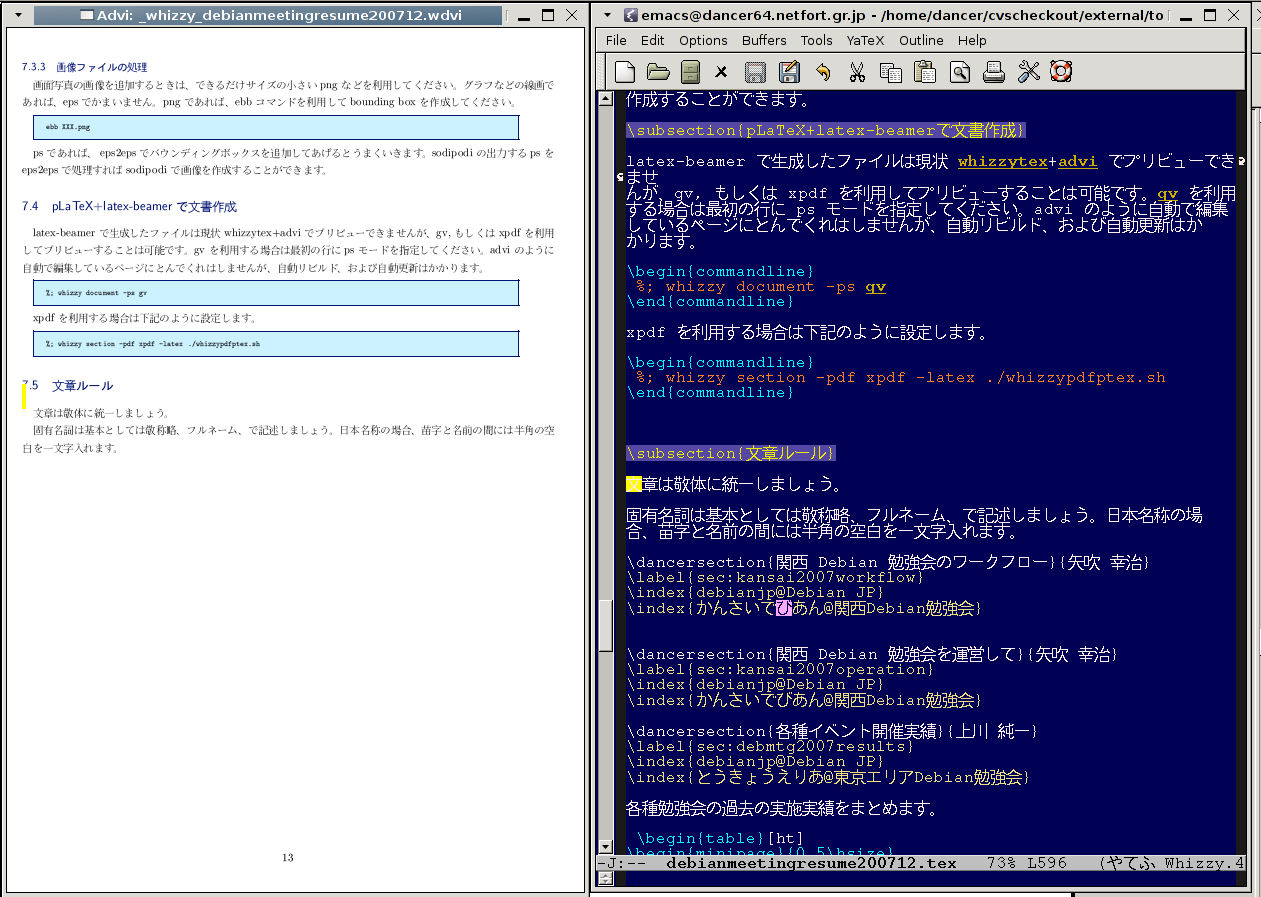
\includegraphics[width=1\hsize]{image200712/whizzytex.png}
\end{frame}


\begin{frame}[containsverbatim]{gitでデータ連携}

\begin{commandline}
 git-clone git://git.debian.org/git/tokyodebian/monthly-report.git
or
 git-clone ssh://ユーザ名@git.debian.org/git/tokyodebian/monthly-report.git

 cd monthly-report.git
 make
 git-diff
 git-commit -a -m 'revised XXX'
 git-pull
 git-push ssh://ユーザ名@git.debian.org/git/tokyodebian/monthly-report.git
\end{commandline}

\end{frame}
\begin{frame}{Q\&A}
 これだけでわからない?
\end{frame}

\emtext{19:20 まで休憩}

\section{}

\emtext{2007年をふりかえる}


\begin{frame}{Debian JP の構成}
\begin{itemize}
 \item Debian JPの会員は開発・翻訳・インフラを担当している人により構成さ
	れています。過去の経緯により、既存の会則・方針では、Debian JP は
	「開発者の会」という位置づけのため、「ユーザ」については Debian
	JP の「会員」ではありません。
 \item 開発者とは Debian JP で開発を行っている人、パッケージ・スポンサー
	されている人、New Maintainer、 Debian Developer などをいいます。
 \item インフラは、Debian JP の運営に必要なインフラで ftp, www, svn, ML,
       LDAP などをいいます。
\end{itemize}

\begin{figure}[h]
\begin{center}
  {\large
 \begin{tabular}[t]{|c|c|c|}
 \hline
 \rotatebox{90}{ユーザ }& \rotatebox{90}{開発者 }&\rotatebox{90}{翻訳者 } \\
 \hline
 \multicolumn{3}{|c|}{インフラ}\\
 \hline
 \end{tabular}
 }
\end{center}
 \caption{Debian JP のメンバー要素分類}
\label{fig:debianjpmemberitem}
\end{figure}
\end{frame}

\begin{frame}{Debian JP の各種会議体}
 \includegraphics[width=1\hsize]{image200712/debianmeetinganddebianjp.eps}
\end{frame}

\begin{frame}{Debian JP の各種会議体}

Debian JP の各種会議体の頻度とメンバー構成

{\scriptsize
\begin{tabular}[t]{|p{6em}|l|p{10em}|p{10em}|}
\hline
会 & 開催頻度 & 目的 & 参加者層 \\
\hline
総会・選挙 & 年一回 & Debian JP 内部の運営方針の策定 & Debian JP 会員 \\
OSC & 年数回 & 新規ユーザ発掘・公報 & OSCの一般参加者 \\
東京エリアDebian勉強会 & 月一回 & Debian 開発者の新規発掘と支援 & Debian の開発者をめざす東京近辺在住の
 メンバー \\
関西Debian勉強会 & 月一回 & Debian ユーザ・開発者の新規発掘と支援 & Debian を使う大阪近辺
	     在住のメンバー\\
IRC定例会議 & 月に二回 & Debian JPの運営に関する情報共有と意思決定 & Debian JP
 会員 \\
\hline
\end{tabular}
}

\hfill{}→こんな感じ?
\end{frame}

\begin{frame}{情報の伝達の流れ}

情報の伝達を整理してみました。

\includegraphics[width=0.7\hsize]{image200712/debianjpandmedia.eps}

\hfill{}→こんな感じ?

\end{frame}

\section{}
\begin{frame}{Debian 勉強会の目的}

\begin{itemize}

 \item Debian Developer (開発者)の育成。

 \item  日本語での開発に関する情報を整理してまとめてアップデートする。

 \item 場所の提供。
\begin{itemize}
 \item 普段ばらばらな人々が face-to-face で出会える。
 \item Debian のためになることを語る。
 \item Debianについて語る場所を提供する。
\end{itemize}

\end{itemize}

\end{frame}

\section{}

\begin{frame}{12月の目的}

 忘年会をするのはなぜか

\begin{itemize}
 \item MJK\\
       →
       \only<2->{\textbf{目的と実績の確認}}
 \item SS\\
       →
       \only<2->{\textbf{将来を想定する}}
 \item KKS\\
       →
       \only<2->{\textbf{計画の確認と修正}}
\end{itemize}
\end{frame}

\begin{frame}{}
 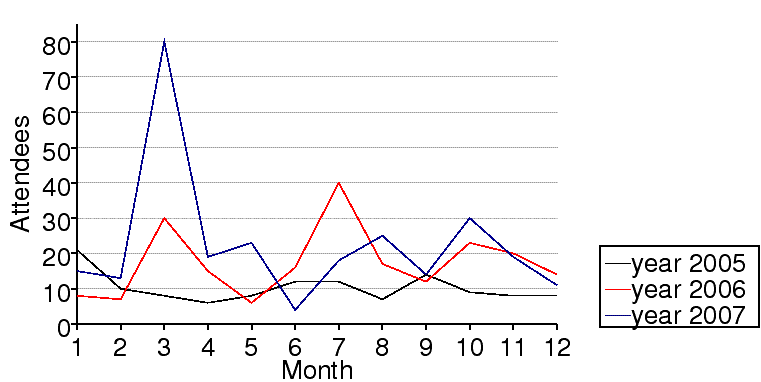
\includegraphics[width=10cm]{image200712/people-chart.png}
\begin{itemize}
 \item 2007年の平均は 18人くらいで、2006年の平均の16人くらいよりは増えて
       いる
 \item 極端に増えているわけではない
\end{itemize}
\end{frame}

\section{}
\begin{frame}{2007年実施状況}
  \begin{tabular}{|l|c|p{10em}|}

 & 参加人数 & 内容\\
 \hline
2007年1月 & 15 & 一年を企画する \\
2007年2月 & 13 & dbs, dpatch\\
2007年3月 & 80 & OSC仮想化 \\
2007年4月 & 19 & quilt, darcs, git\\
2007年5月 & 23 & etch, pbuilder, superh \\
2007年6月 & 4 & エジンバラ開催:Debconf7 実況中継 \\
2007年7月 & 18 & Debconf7 参加報告\\
2007年8月 & 25 & cdn.debian.or.jp \\
2007年9月 & 14 & exim \\
2007年10月 & 30 & OSC Tokyo/Fall(CUPS) \\
2007年11月 & 19 & live-helper, tomoyo linux kernel patch, server\\
2007年12月 & 12? & 忘年会\\
 \hline
  \end{tabular}
\end{frame}

\section{}
\emtext{将来の想定}

\section{}

\begin{frame}

イベントとトレンドの確認

{\tiny
\begin{tabular}[t]{|p{6em}|p{6em}|p{6em}|p{6em}|p{6em}|}
\hline
2005 &2006 &2007 &2008 &2009 \\
\hline
%2005
Debian 勉強会開始、

Wzero3登場、
lantank(SH)ブーム、
黒箱(PPC)、
OpenBlocS(PPC) (2004年?)、

Ubuntu開始、

AMD64が一般的に入手可能に、

gitの登場、
ruby on rails が普及、

光ファイバー普及、

雑誌が消失しはじめ、

スレッドテンプレ登場、

 &
%2006
IntelMacに、coreduoでdual-core CPU に、

glantank(ARM)、
OpenMicroServer(MIPS)、

OpenSolarisが出てDebian/Solaris (Nexenta) 登場、
SparcT1がオープンに、

CC3.0、

Qwik登場(?)、

雑誌が大多数消失、

 &
%2007
VT・AMD-V(仮想化技術)が普及(ML115!)、

黒箱(ARM)、
OpenBlocks(PPC?)、
iPhone登場、
HSDPA 月額5000円くらいに、
google mobile、

VISTAリリース、
Leopardリリース、

GPL3.0、
メモリ2Gとがコモディティーに、
SparcT2がオープン、
ニコニコ動画、
winny でイージスの情報流出、
 &
%2008
FreeBSD7リリース、

Longhornリリースで64bitサーバが常識に、

lennyリリース、

ruby1.9が出ているはず、

Google Android、

OLPC 日本上陸、
eeePC 日本上陸、

imode世代が社会人になる、
パソコンが使えない人が増え携帯に、

J-SOX、
thin-client化、

&
%2009
VISTAが64bitでまともに稼働するようになる、

4GBメモリが普及して家庭でも 64bit OS がポピュラーに、

ruby2が出ているかも、

(Windowsが対応したとして) Trusted Computing が一般に普及してしまう、

携帯電話の普及率が100\%くらいに、

日本DMCA法?、

 \\

\hline
\end{tabular}
 }

2011 アナログ地上波全滅


\end{frame}

\section{}
\begin{frame}{}

%SWOT
{\scriptsize
\begin{tabular}[t]{|p{8em}|p{8em}|p{8em}|p{8em}|}
\hline
できたこと & できなかったこと & チャンスとなるもの & 脅
 威となるもの \\
\hline
%S
OSCきっかけでDebian勉強会に参加できた、
新規の参加メンバーがきている、
謎に包まれたDebian開発者の(魅力的な)実状があきらかに、
濃さやアンドキュメンテッドなところが直接きける、
二年かかったけどetchのリリース、
某所で本を売ることができた、
&
%W

Debconfの誘致ができない、
DEBのパッケージを新規に作りたいができなかった、
女の子メンバーが少ない、
BTSがフレンドリーじゃない、
NMを誰も通過していない、
BSPで集まってもIRCで会話している、

&
%O
仮想化、
Debianがうらにいるものの普及(Ubuntu・Knoppix)、
Debconfが開催できるかも、
世間の各種オープンになっている動き(Solaris・java・ATI)、
GPLv3、
Blogの普及(情報の普及)、
イベントでの告知、
OSCでも興味を引いている、
&
%T
thin-client、
携帯への流出、
会社でDebianが使えなく、
Ubuntu (勝手にメンテナ・ハードウェア認識の良さでのユーザ流出・ファーム
	     ウェアライセンス無視)、
人材の流出(Ubuntu, G社)、
Webの向こう側へのシフト、

\\
\hline
\end{tabular}
}
\end{frame}

\section{}
\begin{frame}{}

% SWOT 2
{\tiny
\begin{tabular}[t]{|p{4em}|p{11em}|p{11em}|p{11em}|}
\hline
 &  & チャンスとなるもの & 脅威となるもの  \\\hline
 & &
%O
仮想化、
Debianがうらにいるものの普及(Ubuntu・Knoppix)、
Debconfが開催できるかも、
世間の各種オープンになっている動き(Solaris・java・ATI)、
GPLv3、
Blogの普及(情報の普及)、
イベントでの告知、
OSCでも興味を引いている、
&
%T
thin-client、
携帯への流出、
会社でDebianが使えなく、
Ubuntu (勝手にメンテナ・ハードウェア認識の良さでのユーザ流出・ファーム
	     ウェアライセンス無視)、
人材の流出(Ubuntu, G社)、
Webの向こう側へのシフト、
\\
\hline
できたこと &
%S

 OSCきっかけでDebian勉強会に参加できた、
 新規の参加メンバーがきている、
 謎に包まれたDebian開発者の(魅力的な)実状があきらかに、
 濃さやアンドキュメンテッドなところが直接きける、
 二年かかったけどetchのリリース、
 某所で本を売ることができた、

&

 認知が重要、広報活動を続ける、

 仮想化をテーマに続ける、

 Debconfを誘致、

 オープンになったものをベースに勉強会を開催、

&

 岩松さんを複数養成、
 thin client でDebianに、
 サーバ側でもDebian稼働へ、
 Ubuntu・Fedoraなどと協調して人を育てる、

 Webを使っているんだからClientはDebianでいいじゃん、
 Live DVD配布してしまう、
 ぐるぐるじるしのDebianを、

\\
\hline

できなかったこと
&
%W
Debconfの誘致ができない、
DEBのパッケージを新規に作りたいができなかった、
女の子メンバーが少ない、
BTSがフレンドリーじゃない、
NMを誰も通過していない、
BSPで集まってもIRCで会話している、

&

開発者育成のプログラム (何を気をつけるか・これはやるべき・やらないべき・パッケージのいじりかたの流れ)、
四国のLinuxユーザを増やす、
女の子を仮想化、Debianの擬人化(なんとかミク)、

&



\\
\hline
\end{tabular}
}

\end{frame}

\emtext{計画の確認と修正}

\section{}

\begin{frame}{}

2008年度も、毎月第3土曜日開催、場所不定。
内容としては、開発者育成連載企画を実施する。

{\scriptsize
\begin{enumerate}
 \item 新年会「気合を入れる」
 \item OSC、
       バージョン管理ツールを使いDebianパッケージを管理する(git)
       アップストリームの扱い(svn/git/cvs)
 \item データだけのパッケージを作成してみる、
       ライセンスの考え方
 \item バイナリ一つのパッケージを作成してみる
       man の書き方(roff or docbook)
 \item バイナリの分けたパッケージの作成。
       バイナリの分け方の考え方、アップグレードなどの運用とか。
 \item パッケージ作成(dpatch/debhelperで作成するパッケージ)
 \item パッケージ作成(kernel patch、kernel module)
、Debconf発表練習
 \item Debconf アルゼンチン、共有ライブラリパッケージ作成

 \item OSC-Fall、
       デーモン系のパッケージの作成、latex、 emacs-lisp、フォントパッケージ
 \item パッケージの cross-compile の方法、amd64 上で i386 のパッケージと
       か、OSC-Fall報告会、Debconf報告会
 \item 国際化 po-debconf / po化 / DDTP
 \item 忘年会
\end{enumerate}
}
\end{frame}

\section{事前課題紹介}
\emtext{事前課題の紹介}
% pre work home work

\begin{frame}{事前課題問題}

「Debian勉強会の目的と照らし合わせて2007年を評価してみた」と「2008年
 のDebian勉強会のために私はこうします」というタイトルで200-800文字程度の
 文章を書いてください。

\end{frame}

% (query-replace "\\subsection" "\\end{frame}\\begin{frame}")
% (query-replace "\\subsubsection" "\\textbf")


\begin{frame}{事前課題提出状況}
ちなみに、2007年の課題の提出状況はこんな感じ
{\scriptsize
\begin{table}[h]
 \begin{center}
  \begin{tabular}{|l|c|c|p{23em}|}
 \hline
 & 参加数 & 提出人数 & 内容\\
 \hline
1月 & 15 & 6 & 今後、勉強会につかう施設を提案してください、2007年の勉強会の各月のアジェンダを提案してください\\
2月 & 13 & 8 & aptに足りなさそうな機能, パッケージングをしてみて感じたこと、または何故パッケージングをしないか\\
3月 & 80 & 6 & 仮想化を実際にこういう利用方法で活用しています\\
4月 & 19 & 14 & 私はバージョン管理システムをこのようにつかっています \\
5月 & 23 & 14 & 「エッチになって困った事」 \\
7月 & 18 & 12 & 今後Debconfを日本で開催するためにDebianの認知度を上げる方法、企業がDebconfのスポンサーになるためには \\
8月 & 25 & 18 & ここ最近 Debian を使っていて ハマったこと/ちょっと
	       感激したこと、apt の sources.list はこう書く\\
9月 & 14 & 7 & 「あなたがDebianで使っている MTA のこだわりの設定」もしくは「Debian
 で利用しているこんな便利な/楽しいメッセージツールあるいは日頃使っていて
 気にかかるメッセージ関連ソフトのこの部分」\\
11月 & 19 & 10 & 「Debian の Live CD ってこんなふうに使ってます」もしく
	   は「ノートPCやデスクトップPCではなく、サーバ機器での Debian
	   に期待するものって何?」\\
12月 & 11 & 11 & 「Debian勉強会の目的と照らし合わせて2007年を評価してみた」と「2008年のDebian勉強会のために私はこうします」\\
 \hline
  \end{tabular}
 \end{center}
\end{table}
}

\end{frame}

\begin{frame}{石原怜美}

\textbf{Debian勉強会の目的と照らし合わせて2007年を評価してみた}

 少ししか参加していないのでなんともいえない、です…
 でも、Debian勉強会のことを知り合いに話したら興味を持ってもらえたので
 自分の中ではよし、とします。

\textbf{2008年のDebian勉強会のために私はこうします}

 実は、地元に帰ってしまうので、私自身は参加できないのですが、
 友人にがんばってもらいます。
 地元でもちょっと普及の努力をしてみようかな…


\end{frame}\begin{frame}{小室 文}
\textbf{Debian勉強会の目的と照らし合わせて2007年を評価してみた}

\begin{description}
 \item[メールでは読み取れない情報について情報共有する場を作る]
これに関してはもっと参加者が分からなかった事などを積極的に聞いたり、ま
 た自分で調べて発表するとか、そういう姿勢が足りなかったと思います。

 \item[Debianの利用方法を整理する場を作る]
 よりよく使う方法と、よりよくする仕組みを作る方法があると思いますが、前
 者にフォーカスしていたので(フォーカスしやすいというのもありますが)、来
 期は2部構成などで、使う方法、作る方法など講義や論議が分かれていたらよい
 かもしれないなーと思いました。
\end{description}
\end{frame}\begin{frame}{小室 文}

\textbf{2008年のDebian勉強会のために私はこうします}

gitを使えるようにします。
Latexでもっと多彩な表現が出来るようにします。
会社の引継ぎをDebian使いにします。
Eximの普及活動もついでにします。
未来のDebian使いを増やします。

\end{frame}\begin{frame}{本庄}

\textbf{「Debian勉強会の目的と照らし合わせて2007年を評価してみた」}

「勉強会の目的」を探してみたのですが、どうも見あたらないようでし
た。東京エリアDebian勉強会のウェブページに、背景として「2005年当
初、東京近辺で、類似の勉強会は存在していませんでした。Debian に
ついて語る場所を提供するため、 Debian 勉強会を開催します。」と書
かれており、これが目的に相当するのではないかと思いますが、語る場
として機能していたと思います。

\textbf{「2008年のDebian勉強会のために私はこうします」}

風邪で休んでしまったこともあったので、風邪ひかない。

\end{frame}\begin{frame}{山本 浩之}

\textbf{「Debian勉強会の目的と照らし合わせて2007年を評価してみた」}

うーむ、2007年の時点では、スーパーハカーにはまだなれていません。

\textbf{「2008年のDebian勉強会のために私はこうします」}

こんなわたくしでもお役に立つなら、お手伝いくらいはします。
ただ、現在何が不足していて、どうお手伝いすればいいのかが分からないです。
「雰囲気作りのために、声を出していこー」と、体育会みたいなノリでいいです
かね?
願わくば、講師ができるぐらいのスーパーハカーになれればいいのですが…。

\end{frame}\begin{frame}{前田耕平}

\textbf{「Debian勉強会の目的と照らし合わせて2007年を評価してみた」}

Debian勉強会の本来の目的というと、Debianの開発者を増やす事ですよね。勉強会として今年を振り返ると、年初の勉強会でまずは裾野を広げ、分母を増やして開発者候補を増やそうという目標になった記憶があります。その点については新規参加者が増えたので成果はあったと思います。
自分自身を振り返ると今年は昨年参加し始めたころからますます『お客さん』化しているなと反省。おまけに、未だ自宅鯖もSargeのままだし。

\end{frame}\begin{frame}{前田耕平}
\textbf{「2008年のDebian勉強会のために私はこうします」}

初心に返り、当初勉強会に参加しようと思ったきっかけである、HobbitのDebianの公式パッケージ化を目指して、ライセンスあたりが面倒でいつも中途半端になっているDebianパッケージの勉強をちゃんとします。ほいで、完全に放置状態にしてしまった査読を一日10分でもやります。
その前に年内には、この帰っても休みでも仕事な状態を脱しないと。

\end{frame}\begin{frame}{小林儀匡}

\textbf{ Debian勉強会の目的と照らし合わせて2007年を評価してみた}

今年の勉強会の目的は、(女子高生などはともかく) 参加者を増やすことだった気がするので、それはクリアできたのではないかと思います。
ただ、参加者を増やしたことが広義の開発者 (公式開発者でなくてもパッケージ管理や翻訳に携わっている人を含む) の増加に繋がっているかといえば、間違いなくNoでしょう。
参加者がガリガリとDebianパッケージのメンテナンスをするような姿を
想像する当初の目的とはずれてきている気がします。
\end{frame}\begin{frame}{小林儀匡}

\textbf{2. 2008年のDebian勉強会のために私はこうします}

こんなところでしょうか。
\begin{itemize}
 \item  Debian勉強会出身の公式開発者の一人になるべくNew Maintainer (NM) processを進めます
 \item  builddやdakについて勉強して皆さんの前で話をできるようになります。
 \item  もし翻訳関連で何か話すべきことがあれば話をします。
\end{itemize}

\end{frame}\begin{frame}{吉田@板橋}

\textbf{Debian勉強会の目的と照らし合わせて2007年を評価してみた}

Debian勉強会の目的とは\url{http://tokyodebian.alioth.debian.org/}から
「Debian について語る場所を提供するため、 Debian 勉強会を開催します。」と
判断しました。

2007年の東京エリアDebian勉強会は、上川さん、岩松さんの毎回の勉強会での
Debianの深いお話、イベントレポート、やまねさんの初心者をDebianに引き込む
プレゼンなどなど、素晴らしいお話を聞ける勉強会でした。元は東京で始まった、
Debian勉強会は関西でも定期的に開催されるようになり、荻窪、代々木、新宿
(OSC)、イギリス エジンバラ、IRC開催等、地域や国、3次元の枠を超え、活動的
ですばらしいです。

\end{frame}\begin{frame}{吉田@板橋}

\textbf{2008年のDebian勉強会のために私はこうします}

私はごくごく一般人のため、Debian勉強会への貢献は難しいとは思いますが、イ
ベントでDebian勉強会関連の冊子の配布に協力させていただいたり、別の勉強会
主催のインストールパーティで何も知らない一般人のPC(のVM上)にDebianをイン
ストールするなどひっそりと協力させていただこうと思います。

\end{frame}\begin{frame}{あけど}


\textbf{「Debian勉強会の目的と照らし合わせて2007年を評価してみた」}

今年1年を振り返って、自分に何が出来たのか考えてみました。

{\scriptsize
 \begin{itemize}
 \item  1月一年の計画を立てた。
 \item  2月aptを少し勉強した。
 \item  3月仮想化を少し勉強した。
 \item  4月バージョン管理システムを少し勉強した。 MacにDebianをインストールしてみた。
 \item  5月Etchを少し勉強した。 管理しているDebianマシンをEtchにしてみた。
 \item  6月エジンバラに行ってるメンバーとIRCしようとして挫折
 \item  7月(お休み)
 \item  8月cdn を少し勉強した。BSPに参加、少し査読。・・・って残りがまだあった! orz
 \item  9月(お休み)
 \item  10月OSCで盛り上がった。
 \item  11月(お休み)
 \end{itemize}
}
後半は何かと忙しくて時間が取れなかったこともあり、殆ど何も出来てません。
点数でいえば20点くらい?
やりたかった事は何もできてませんので、
来年はもう少し計画的にやって何か出来たという風にしたいです。

\end{frame}\begin{frame}{あけど}
\textbf{「2008年のDebian勉強会のために私はこうします」}

今年の反省を踏まえ、自分に出来そうなことをやっていきたいです。
1つは、マニュアルのレシピ化というのを考えています。
いわゆる事例集のようなものですが、
各コマンドの実行例とコマンドオプションのポイントといったものを
まとめてみたいと思います。
来年の後半には何らかの発表が出来るようにしたいと思います。

\end{frame}\begin{frame}{山本 琢}

今年勉強会で実現できたこと:\\
 オープンソースのカルチャーに触れて、オープンソース開発に興味を持てた。

来年勉強会で実現したいこと:\\
 実際にオープンソース開発プロジェクトに貢献(パッチを投げられる)し、その
過程や成果についての報告や、アドバイスが受けれるようにしたい。

\end{frame}\begin{frame}{キタハラ}

\textbf{「Debian勉強会の目的と照らし合わせて2007年を評価してみた」}

  お題を見て、改めて勉強会のWebページを見たの
ですが、「背景」はありますが「目的」はないですね。
(見落としている?) 「背景」にある「Debian につい
て語る場所を提供するため」というのが目的だとすると、
有識者の方に大いに語って戴いて、(私の理解の範囲外
なものもありましたが)多くの有用な知識を得ることが
出来て、私にとっては(勉強会の後の懇親会も含めて)
大変有意義であったと思います。

  真の目的(?)にはまったく貢献していませんが、
無能が故ということでお許しください。

\end{frame}\begin{frame}{上川 純一}

Debian勉強会の目的と照らし合わせて2007年を評価してみたところ、
自由の戦士(Debian Developer)を量産することが目的だったのに、第3次自由の
戦士量産計画は成果を出せずに終了しました。ふがいない。

「2008年のDebian勉強会のために私はこうします」という観点からいうと、
もしかして、NMキュー通過のためのブートキャンプなどをすればよいんじゃない
か?

\end{frame}



\emtext{2008年を計画する}


\section{}
\begin{frame}{宴会場所}

\begin{itemize}
 \item 宴会場所\\
       本日の宴会は「刻」です。
  参加者は1Fに集合し、全員で移動しましょう。
 \item 片付け\\
       部屋を片付けるのにご協力ください。
\end{itemize}


\end{frame}

\end{document}

;;; Local Variables: ***
;;; outline-regexp: "\\([ 	]*\\\\\\(documentstyle\\|documentclass\\|emtext\\|section\\|begin{frame}\\)\\*?[ 	]*[[{]\\|[]+\\)" ***
;;; End: ***
